\section{Consuntivo di periodo}
		In questa sezione verranno riportati il consuntivo per le varie fasi di lavoro, considerando le ore sostenute da ogni componente per ruolo. Il bilancio potrà essere:
		\begin{itemize}
			\item \textbf{positivo:} se sono state necessarie meno ore rispetto a quelle preventivate;	 
			\item \textbf{paritario:} se le ore preventivate rispettano quelle effettive;	 
			\item \textbf{negativo:} se sono state necessarie più ore rispetto a quelle preventivate.
		\end{itemize}
	\subsection{Fase di analisi dei requisiti}
		Le ore di lavoro svolto in questo periodo sono di solo investimento e destinate all'apprendimento personale. Di conseguenza queste ore non sono rendicontate. 
		\subsubsection{Prospetto orario}
			Nella tabella in seguito viene illustrato il cambiamento nel numero d'ore di ogni persona, per ogni ruolo ricoperto:
			
			\rowcolors{2}{white}{lightest-grayest}
			\begin{longtable}{|c|c|c|c|c|c|c|c}
				\hline
				\rowcolor{lighter-grayer}
				\textbf{Nome} & \textbf{Re} & \textbf{Am} & \textbf{An} & \textbf{Pg}  & \textbf{Pr}   & \textbf{Ve} & \textbf{Totale} \\
				\hline
				\endfirsthead
				
				\hline
				Giuseppe Vito Bitetti 		& 0 & 8(-1) & 10(+1) & 0 & 0 & 12 & 30\\
				\hline
				\hline
				Lorenzo Dei Negri			 & 6(-2) & 0 & 14(+1) & 0 & 0 & 10(+1) & 30\\
				\hline
				\hline
				Nicolò Frison 					& 0 & 8(-2) & 9(+1) & 0 & 0 & 13(+1) & 30\\
				\hline
				\hline
				Fouad Mouad 				& 0 & 7 & 11 & 0 & 0 & 12 & 30\\
				\hline
				\hline
				Mariano Sciacco 			& 8 & 0 & 12 & 0 & 0 & 10 & 30\\
				\hline
				\hline
				Alessandro Tommasin    & 9(-2) & 0 & 12(+2) & 0 & 0 & 9 & 30\\
				\hline
				\hline
				Giovanni Vidotto 			& 0 & 6(-1) & 9(+1) & 0 & 0 & 15 & 30\\
				\hline 
				\caption{Tabella contenente il prospetto orario preventivato per la fase di analisi dei requisiti}
			\end{longtable}
			\pagebreak	
			
			La tabella può essere riassunta nel seguente istogramma:
			
			\begin{figure}[H]
				\centering
				\includegraphics[width=0.8\linewidth]{images/consuntivo/analisiCons1.png}
				\caption{Grafico consuntivo ore/ruolo componenti nella fase di analisi dei requisiti}
				\label{fig:consuntivo grafico suddivisione ruoli fase analisi dei requisiti}
			\end{figure}
			
		\subsubsection{Prospetto economico}
			In base al prospetto orario, quello economico sarà il seguente: 
			
			\rowcolors{2}{white}{lightest-grayest}
			\begin{longtable}{|c|c|c|c|c|c|c|c}
				\hline
				\rowcolor{lighter-grayer}
				\textbf{Ruolo} & \textbf{Ore} & \textbf{Costo in €} \\
				\hline
				\endfirsthead
				
				\hline
				Responsabile & 23 (-4) & 690,00 (-120,00)\\
				\hline
				\hline
				Amministratore & 29 (-4) & 580,00 (-80,00)\\
				\hline
				\hline
				Analista & 77 (+6) & 1.925,00 (+150,00)\\
				\hline
				\hline
				Progettista & - & -\\
				\hline
				\hline
				Programmatore & - & -\\
				\hline
				\hline
				Verificatore & 81 (+2) & 1.215,00 (+30,00)\\
				\hline
				\textbf{Totale} & 210 & 4.410,00 (-20,00)\\
				\hline
				\caption{Tabella contenente il prospetto economico in riferimento al prospetto orario}
			\end{longtable}
			\pagebreak
			
			La tabella può essere riassunta nel seguente areogramma:
			\begin{figure}[H]
				\centering
				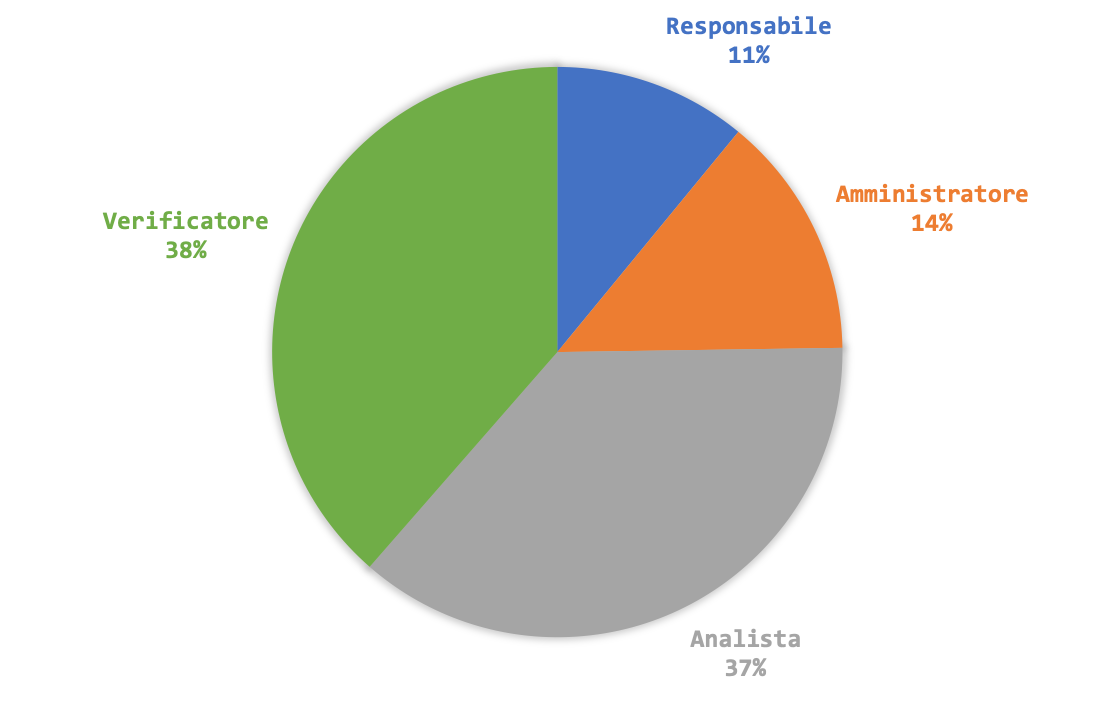
\includegraphics[width=0.8\linewidth]{images/consuntivo/analisiCons2.png}
				\caption{Grafico percentuale ore/ruolo nella fase di analisi dei requisiti}
				\label{fig:consuntivo2 grafico costi ruolo fase analisi dei requisiti}
			\end{figure}
		
		

		\subsection{Fase di consolidamento dei requisiti}
		Le ore di lavoro svolte in questo periodo sono volte alla preparazione della presentazione e alla revisione dei requisiti individuati. 
		\subsubsection{Prospetto orario}
			Nella tabella in seguito viene illustrato il cambiamento nel numero d'ore di ogni persona, per ogni ruolo ricoperto:
			
			\rowcolors{2}{lightest-grayest}{white}
			\begin{longtable}{|c|c|c|c|c|c|c|c}
				\hline
				\rowcolor{lighter-grayer}
				\textbf{Nome} & \textbf{Re} & \textbf{Am} & \textbf{An} & \textbf{Pg}  & \textbf{Pr}   & \textbf{Ve} & \textbf{Totale} \\
				\hline
				\endfirsthead
				
				\hline
				Giuseppe Vito Bitetti 	& 0 & 0 & 5 & 0 & 0 & 0 & 5\\
				\hline
				\hline
				Lorenzo Dei Negri	 	& 0 & 5 & 0 & 0 & 0 & 0 & 5\\
				\hline
				\hline
				Nicolò Frison			   & 0 & 0 & 0 & 0 & 0 & 5 & 5\\
				\hline
				\hline
				Fouad Mouad 			& 1 (-1) & 0 & 1 (+1) & 0 & 0 & 3 & 5\\
				\hline
				\hline
				Mariano Sciacco		 	& 0 & 0 & 3 & 0 & 0 & 2 & 5\\
				\hline
				\hline
				Alessandro Tommasin & 0 & 0 & 5 (+1) & 0 & 0 & 0 (-1) & 5\\
				\hline
				\hline
				Giovanni Vidotto 		 & 2 & 0 & 0 & 0 & 0 & 3 & 5\\
				\hline 
				\textbf{Totale} 			& 3 (-1) &  5 & 14 (+2) & 0 & 0 & 13 (-1) & 35\\
				\hline
				\caption{Tabella contenente il prospetto orario preventivato per la fase di consolidamento dei requisiti}
			\end{longtable}
			\pagebreak	
			
			La tabella può essere riassunta nel seguente istogramma:
			
			\begin{figure}[H]
				\centering
				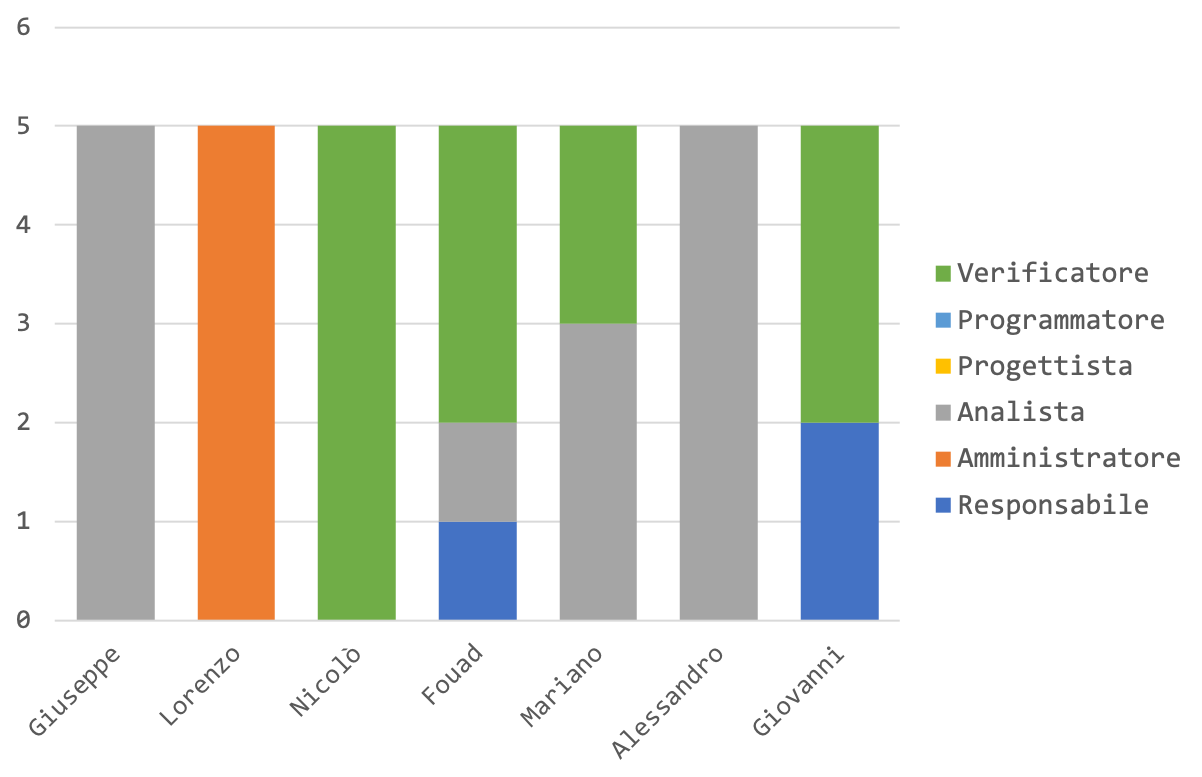
\includegraphics[width=0.8\linewidth]{images/consuntivo/ConsReqCons.png}
				\caption{Grafico consuntivo ore/ruolo componenti della fase di consolidamento dei Requisiti}
				\label{fig:consuntivo grafico suddivisione ruoli fase di consolidamento dei requisiti}
			\end{figure}
			
		\subsubsection{Prospetto economico}
			In base al prospetto orario, quello economico sarà il seguente: 
			
			\rowcolors{2}{white}{lightest-grayest}
			\begin{longtable}{|c|c|c|c|c|c|c|c}
				\hline
				\rowcolor{lighter-grayer}
				\textbf{Ruolo} & \textbf{Ore} & \textbf{Costo in €} \\
				\hline
				\endfirsthead
				
				\hline
				Responsabile & 3 (-1) & 90,00 (-30,00)\\
				\hline
				\hline
				Amministratore & 5 & 100,00\\
				\hline
				\hline
				Analista & 14 (+2) & 350,00 (+50,00)\\
				\hline
				\hline
				Progettista & - & -\\
				\hline
				\hline
				Programmatore & -  & -\\
				\hline
				\hline
				Verificatore & 13 (-1) & 195,00 (-15,00)\\
				\hline
				\textbf{Totale} & 35 & 735,00 (+5,00)\\
				\hline
				\caption{Tabella contenente il prospetto economico in riferimento al prospetto orario}
			\end{longtable}
			\pagebreak
			
			La tabella può essere riassunta nel seguente areogramma:
			\begin{figure}[H]
				\centering
				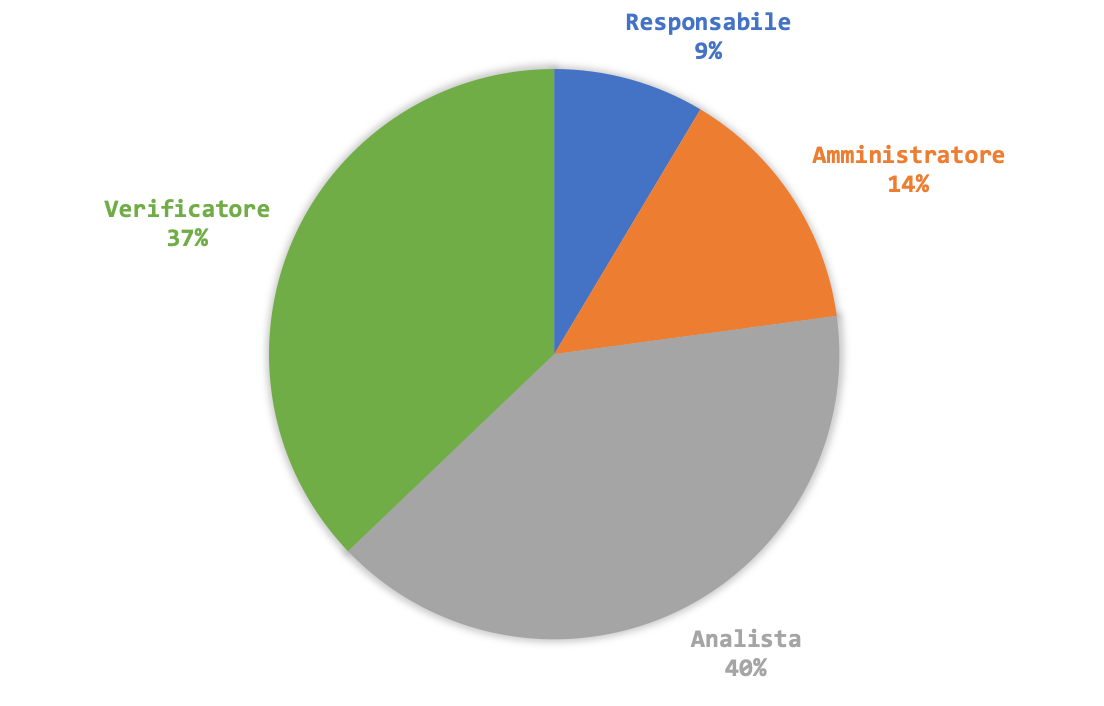
\includegraphics[width=0.8\linewidth]{images/consuntivo/ConsReqCons2.png}
				\caption{Grafico percentuale ore/ruolo nella fase di consolidamento dei requisiti}
				\label{fig:consuntivo grafico costi ruolo fase di consolidamento dei requisiti}
			\end{figure}
		
		\subsubsection*{Conclusioni }
			In questa fase il gruppo ha investito il numero di ore che erano state preventivate. È stato necessario però svolgere alcuni cambiamenti nella suddivisione oraria per ruolo, in particolare:
			\begin{itemize}
				\item \textbf{responsabile:} sono state impiegate meno ore rispetto a quelle preventivate in quanto nella pianificazione del lavoro e nella stesura del piano di progetto sono state riscontrate meno difficoltà del previsto;	 
				\item \textbf{amministratore:} dal momento che i software per la gestione del progetto sono stati individuati e configurati fin da subito e che i documenti sono stati ben strutturati in poco tempo, anche in questo caso sono state impiegate meno ore rispetto a quelle preventivate;	 
				\item \textbf{analista:} per questo ruolo è stato necessario spendere qualche ora in più in quanto alcuni requisiti, per una corretta comprensione, hanno richiesto una delucidazione esterna con i proponenti del progetto, avvenuta con alcune difficoltà di comunicazione;
				\item \textbf{verificatore:} poiché alcuni requisiti sono stati individuati tardivamente e di conseguenza per l'aggiunta di contenuti nel documento di analisi dei requisiti è stato necessario usufruire di qualche ora in più per controllare nuovamente il documento.
			\end{itemize}
			Alla luce dei cambiamenti effettuati il risultato è che il gruppo ha risparmiato 15,00 € investendo le stesse ore preventivate.

			

		\subsection{Fase di progettazione della technology baseline}
		Le ore di lavoro svolte in questo periodo sono volte alla progettazione della \textit{technology baseline} e alla realizzazione della \glock{proof of concept}. 
		\subsubsection{Prospetto orario}
			Nella tabella in seguito viene illustrato il cambiamento nel numero d'ore di ogni persona, per ogni ruolo ricoperto:
			
			\rowcolors{2}{lightest-grayest}{white}
			\begin{longtable}{|c|c|c|c|c|c|c|c}
				\hline
				\rowcolor{lighter-grayer}
				\textbf{Nome} & \textbf{Re} & \textbf{Am} & \textbf{An} & \textbf{Pg}  & \textbf{Pr}   & \textbf{Ve} & \textbf{Totale} \\
				\hline
				\endfirsthead
				\hline
				Giuseppe Vito Bitetti & 2 (-1) & 0 & 7 & 0 & 0 & 4 (+1) & 13\\
				\hline
				\hline
				Lorenzo Dei Negri & 0 & 5 & 1 & 5 & 0 & 2 & 13\\
				\hline
				\hline
				Nicolò Frison & 0 & 3 & 5 & 5 & 0 & 0 & 13\\
				\hline
				\hline
				Fouad Mouad & 0 & 4 & 3 & 2 & 0 & 4 & 13 \\
				\hline
				\hline
				Mariano Sciacco & 3 & 0 & 1 & 9 & 0 & 0 & 13\\
				\hline
				\hline
				Alessandro Tommasin & 0 & 4 & 6 & 0 & 0 & 3  & 13\\
				\hline
				\hline
				Giovanni Vidotto & 2 & 0 & 5 & 2 & 0 & 4 & 13\\
				\hline 
				\textbf{Totale} & 7 (-1) &  16 & 28 & 23 & 0 & 17 (+1) & 91 \\
				\hline
				
				\caption{Tabella contenente il prospetto orario preventivato per la fase di progettazione della technology baseline}
			\end{longtable}
			
			La tabella può essere riassunta nel seguente istogramma:
			
			\begin{figure}[H]
				\centering
				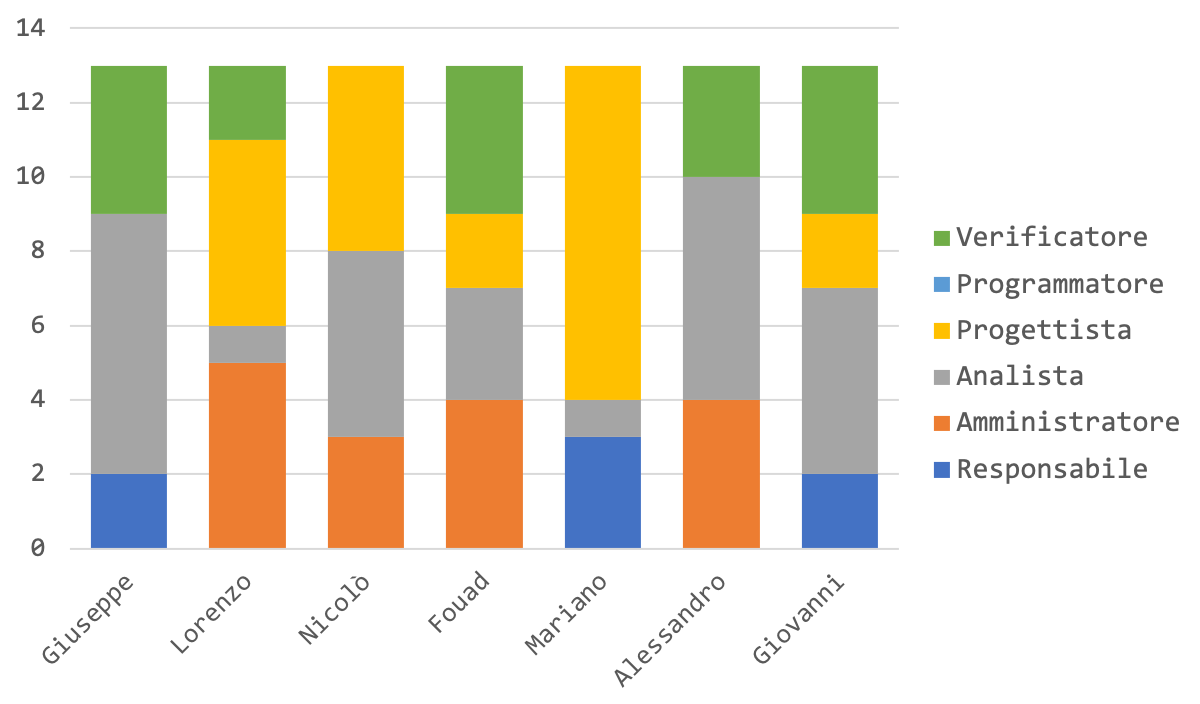
\includegraphics[width=0.8\linewidth]{images/consuntivo/ConsCorrez1.png}
				\caption{Grafico consuntivo ore/ruolo componenti della fase di progettazione della technology baseline}
				\label{fig:consuntivo grafico suddivione ruoli fase di progettazione della technology baseline}
			\end{figure}
		\pagebreak
			
		\subsubsection{Prospetto economico}
			In base al prospetto orario, quello economico sarà il seguente: 
			
			\rowcolors{2}{white}{lightest-grayest}
			\begin{longtable}{|c|c|c|c|c|c|c|c}
				\hline
				\rowcolor{lighter-grayer}
				\textbf{Ruolo} & \textbf{Ore} & \textbf{Costo in €} \\
				\hline
				\endfirsthead
				\hline
			Responsabile 	    & 7 (-1) & 210,00 (-30,00)\\
			\hline 
			\hline
			Amministratore	  & 16 & 320,00\\
			\hline
			\hline
			Analista 				& 28 & 700,00\\
			\hline
			\hline
			Progettista 		  & 23 & 506,00\\
			\hline
			\hline
			Programmatore 	 & 0 & 0,00\\
			\hline
			\hline
			Verificatore 		  & 17 (+1) & 255,00 (+15,00)\\
			\hline
			\textbf{Totale} 	& 91 & 1.991 (-15,00)\\
			\hline
				
				\caption{Tabella contenente il prospetto economico in riferimento al prospetto orario}
			\end{longtable}
			
			La tabella può essere riassunta nel seguente areogramma:
			\begin{figure}[H]
				\centering
				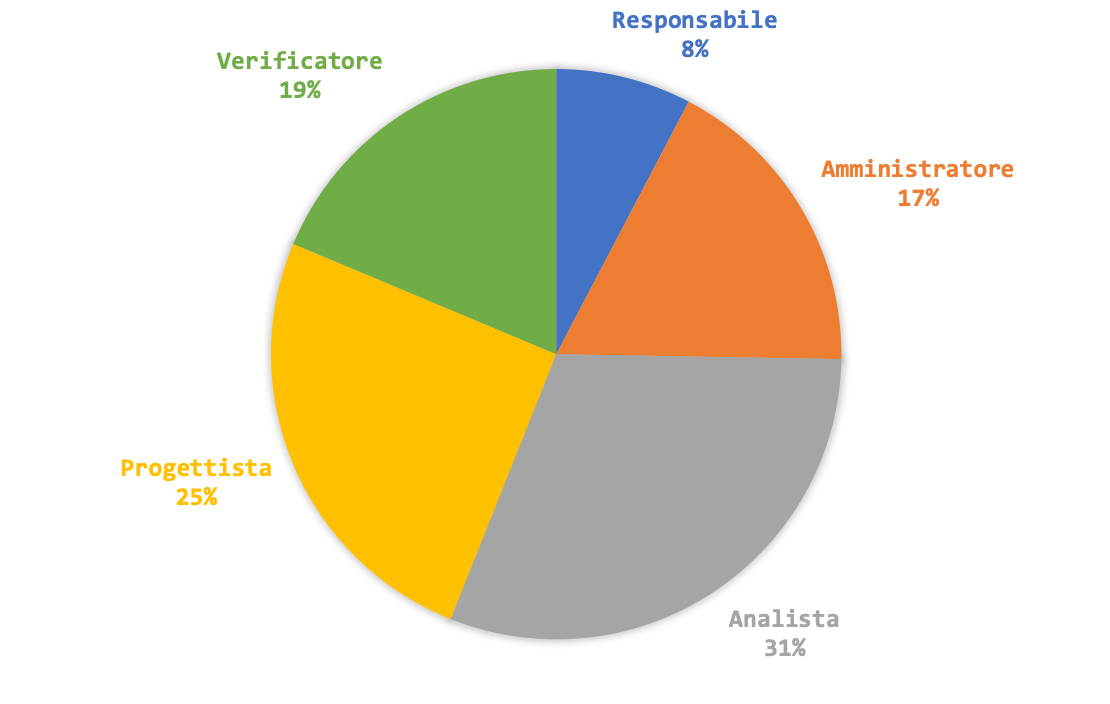
\includegraphics[width=0.8\linewidth]{images/consuntivo/ConsCorrez2.png}
				\caption{Grafico percentuale ore/ruolo nella fase di progettazione della technology baseline}
				\label{fig:consuntivo grafico costi ruolo fase progettazione della technology baseline}
			\end{figure}

		\subsubsection*{Conclusioni}
			Durante la fase di progettazione della technology baseline il gruppo ha lavorato mantenendo il numero di ore che erano state preventivate. È stato necessario però svolgere alcuni cambiamenti nella suddivisione oraria per ruolo, in particolare:
			\begin{itemize}
				\item \textbf{:} 
			\end{itemize}
			Alla luce dei cambiamenti effettuati il risultato è che il gruppo ha ... investendo le stesse ore preventivate.
		

		\subsection{Preventivo a finire}
			A seguito dei cambiamenti riportati .	
		
				
		
		\subsection{Incremento I}
		Le ore di lavoro svolte in questo periodo sono volte alla configurazione dei container e dell'immagine \glock{Docker} di Kafka. 
		\subsubsection{Prospetto orario}
			Nella tabella in seguito viene illustrato il cambiamento nel numero d'ore di ogni persona, per ogni ruolo ricoperto:
			
			\rowcolors{2}{lightest-grayest}{white}
			\begin{longtable}{|c|c|c|c|c|c|c|c}
				\hline
				\rowcolor{lighter-grayer}
				\textbf{Nome} & \textbf{Re} & \textbf{Am} & \textbf{An} & \textbf{Pg}  & \textbf{Pr}   & \textbf{Ve} & \textbf{Totale} \\
				\hline
				\endfirsthead
				\hline
				Giuseppe Vito Bitetti & 0 & 0 & 3 & 0 & 2 & 0 & 5\\
				\hline
				\hline
				Lorenzo Dei Negri & 0 & 0 & 0 & 1 (-1) & 0 & 4 (+1) & 5\\
				\hline
				\hline
				Nicolò Frison & 0 & 2 (-1) & 0 & 0 & 0 & 3(+1) & 5\\
				\hline
				\hline
				Fouad Mouad & 3 & 0 & 2 & 0 & 0 & 0 & 5\\
				\hline
				\hline
				Mariano Sciacco & 0 & 0 & 0 & 3 & 2 & 0 & 5\\
				\hline
				\hline
				Alessandro Tommasin & 0 & 2 & 0 & 3 & 0 & 0 & 5\\
				\hline
				\hline
				Giovanni Vidotto & 2 & 0 & 0 & 0 & 4 & 1 & 5\\
				\hline 
				\textbf{Totale} & 3 &  4 (-1) & 5 & 7 (-1) & 8 & 8 (+2) & 35\\
				\hline 
				
				\caption{Tabella contenente il prospetto orario preventivato per l'incremento I}
			\end{longtable}
			
			La tabella può essere riassunta nel seguente istogramma:
			
			\begin{figure}[H]
				\centering
				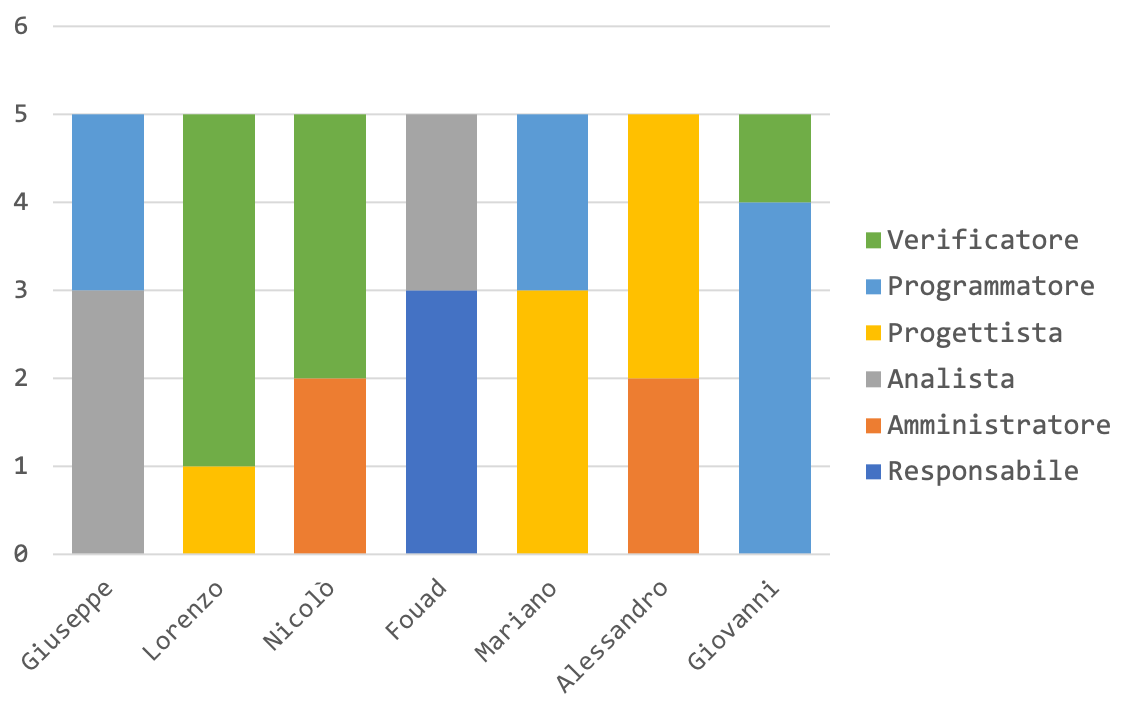
\includegraphics[width=0.8\linewidth]{images/consuntivo/ConsIncr1-1.png}
				\caption{Grafico consuntivo ore/ruolo componenti dell'incremento I}
				\label{fig:consuntivo grafico suddivione ruoli incremento I}
			\end{figure}
		
		\pagebreak
			
		\subsubsection{Prospetto economico}
			In base al prospetto orario, quello economico sarà il seguente: 
			
			\rowcolors{2}{white}{lightest-grayest}
			\begin{longtable}{|c|c|c|c|c|c|c|c}
				\hline
				\rowcolor{lighter-grayer}
				\textbf{Ruolo} & \textbf{Ore} & \textbf{Costo in €} \\
				\hline
				\endfirsthead
				\hline
			Responsabile 	    & 3 & 90,00\\
			\hline 
			\hline
			Amministratore	  & 4 (-1)& 80,00 (-20,00)\\
			\hline
			\hline
			Analista 				& 5 & 125,00\\
			\hline
			\hline
			Progettista 		  & 7 (-1) & 154,00 (-22,00)\\
			\hline
			\hline
			Programmatore 	 & 8 & 120,00\\
			\hline
			\hline
			Verificatore 		  & 8 (+2) & 120,00 (+30,00)\\
			\hline
			\textbf{Totale} 	& 35 & 689,00 (-12,00)\\
			\hline
				
				\caption{Tabella contenente il prospetto economico in riferimento al prospetto orario}
			\end{longtable}
			
			La tabella può essere riassunta nel seguente areogramma:
			\begin{figure}[H]
				\centering
				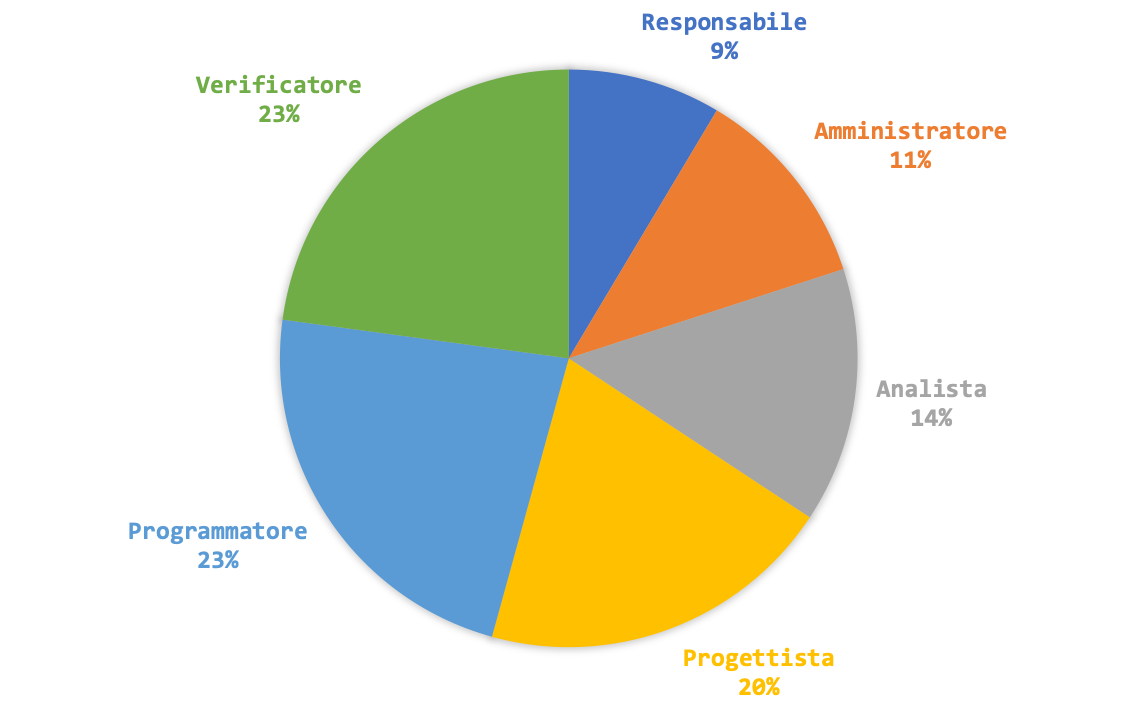
\includegraphics[width=0.8\linewidth]{images/consuntivo/ConsIncr1-2.png}
				\caption{Grafico percentuale ore/ruolo nell'incremento I}
				\label{fig:consuntivo grafico costi ruolo incremento I}
			\end{figure}
			\pagebreak

		\subsubsection*{Conclusioni}
			Durante l'incremento I il gruppo ha lavorato mantenendo il numero di ore che erano state preventivate. È stato necessario però svolgere alcuni cambiamenti nella suddivisione oraria per ruolo, in particolare:
			\begin{itemize}
				\item \textbf{:} 
			\end{itemize}
			Alla luce dei cambiamenti effettuati il risultato è che il gruppo ha ... investendo le stesse ore preventivate.
		

		\subsection{Preventivo a finire}
			A seguito dei cambiamenti riportati .	
		

		\subsection{Incremento II }
		Le ore di lavoro svolte in questo periodo sono volte alla creazione della struttura base del \glock{gateway} ed alla decisione della struttura JSON dei dati da inviare a Kafka. Verrà inoltre implementato un primo protocollo di comunicazione.
		\subsubsection{Prospetto orario}
			Nella tabella in seguito viene illustrato il cambiamento nel numero d'ore di ogni persona, per ogni ruolo ricoperto:
			
			\rowcolors{2}{lightest-grayest}{white}
			\begin{longtable}{|c|c|c|c|c|c|c|c}
				\hline
				\rowcolor{lighter-grayer}
				\textbf{Nome} & \textbf{Re} & \textbf{Am} & \textbf{An} & \textbf{Pg}  & \textbf{Pr}   & \textbf{Ve} & \textbf{Totale} \\
				\hline
				\endfirsthead
				\hline
				Giuseppe Vito Bitetti  & 1 & 0 & 0 & 3 & 1 (+1) & 1 (-1) & 6\\
				\hline
				\hline
				Lorenzo Dei Negri      & 0 & 0 & 0 & 0 & 3 & 3 & 6 \\
				\hline
				\hline
				Nicolò Frison 			  & 3 & 0 & 0 & 0 & 3 & 0 & 6 \\
				\hline
				\hline
				Fouad Mouad 			& 0 & 3 & 2 (-1) & 1 (+1) & 0 & 0 & 6 \\
				\hline
				\hline
				Mariano Sciacco			 & 0 & 0 & 0 & 2 & 0 & 4 & 6 \\
				\hline
				\hline
				Alessandro Tommasin & 0 & 1 & 0 & 0 & 5 & 0 & 6 \\
				\hline
				\hline
				Giovanni Vidotto 		& 0 & 2 & 0 & 4 & 0 & 0 & 6\\
				\hline 
				\textbf{Totale} 		   & 4 &  6 & 2 (-1) & 11 (+1) & 12 (+1) & 8 (-1) & 42\\
				\hline 
				
				\caption{Tabella contenente il prospetto orario preventivato per l'incremento II}
			\end{longtable}
			
			La tabella può essere riassunta nel seguente istogramma:
			
			\begin{figure}[H]
				\centering
				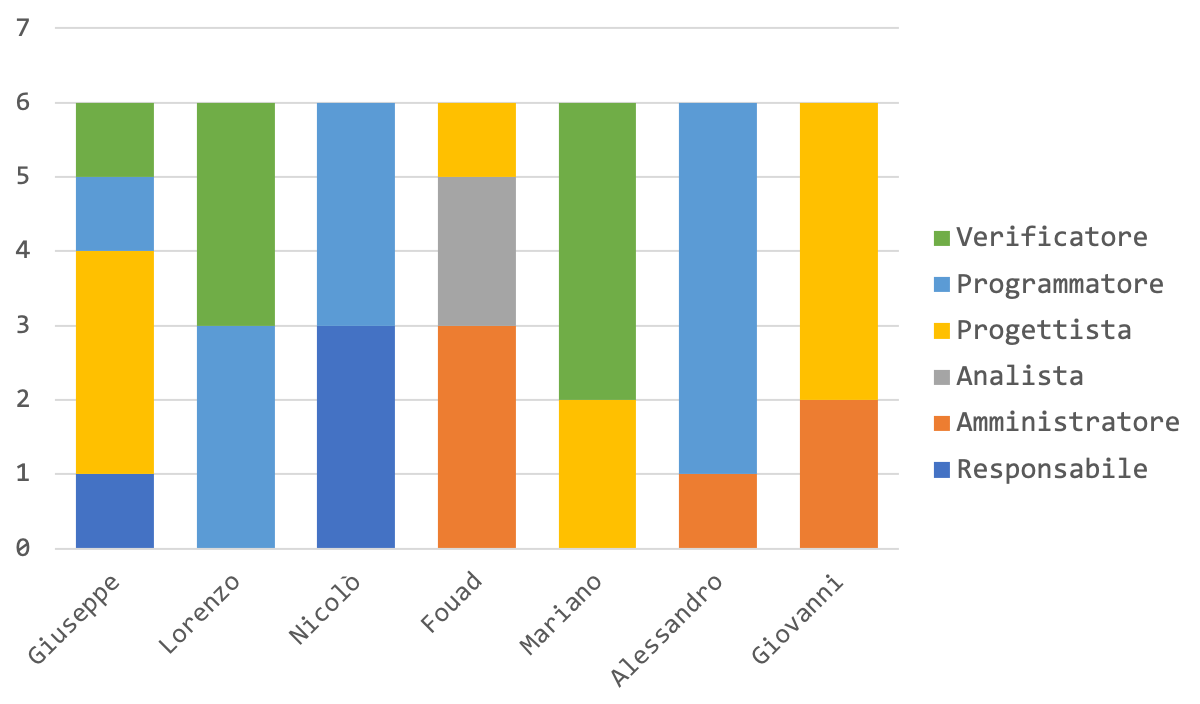
\includegraphics[width=0.8\linewidth]{images/consuntivo/ConsIncr2-1.png}
				\caption{Grafico consuntivo ore/ruolo componenti dell'incremento II}
				\label{fig:consuntivo grafico suddivione ruoli incremento II}
			\end{figure}
			\pagebreak
			
		\subsubsection{Prospetto economico}
			In base al prospetto orario, quello economico sarà il seguente: 
			
			\rowcolors{2}{white}{lightest-grayest}
			\begin{longtable}{|c|c|c|c|c|c|c|c}
				\hline
				\rowcolor{lighter-grayer}
				\textbf{Ruolo} & \textbf{Ore} & \textbf{Costo in €} \\
				\hline
				\endfirsthead
				\hline
			Responsabile 	    & 4 & 120,00\\
			\hline 
			\hline
			Amministratore	  & 6 & 120,00\\
			\hline
			\hline
			Analista 				& 2 (-1) & 50,00 (-25,00) \\
			\hline
			\hline
			Progettista 		  & 10 (+1) & 220,00 (+22,00)\\
			\hline
			\hline
			Programmatore 	 & 12 (+1) & 180,00 (+15,00)\\
			\hline
			\hline
			Verificatore 		  & 8 (-1) & 120,00 (-15,00) \\
			\hline
			\textbf{Totale} 	& 42 & 810,00 (-3,00) \\
			\hline
				
				\caption{Tabella contenente il prospetto economico in riferimento al prospetto orario}
			\end{longtable}
			
			La tabella può essere riassunta nel seguente areogramma:
			\begin{figure}[H]
				\centering
				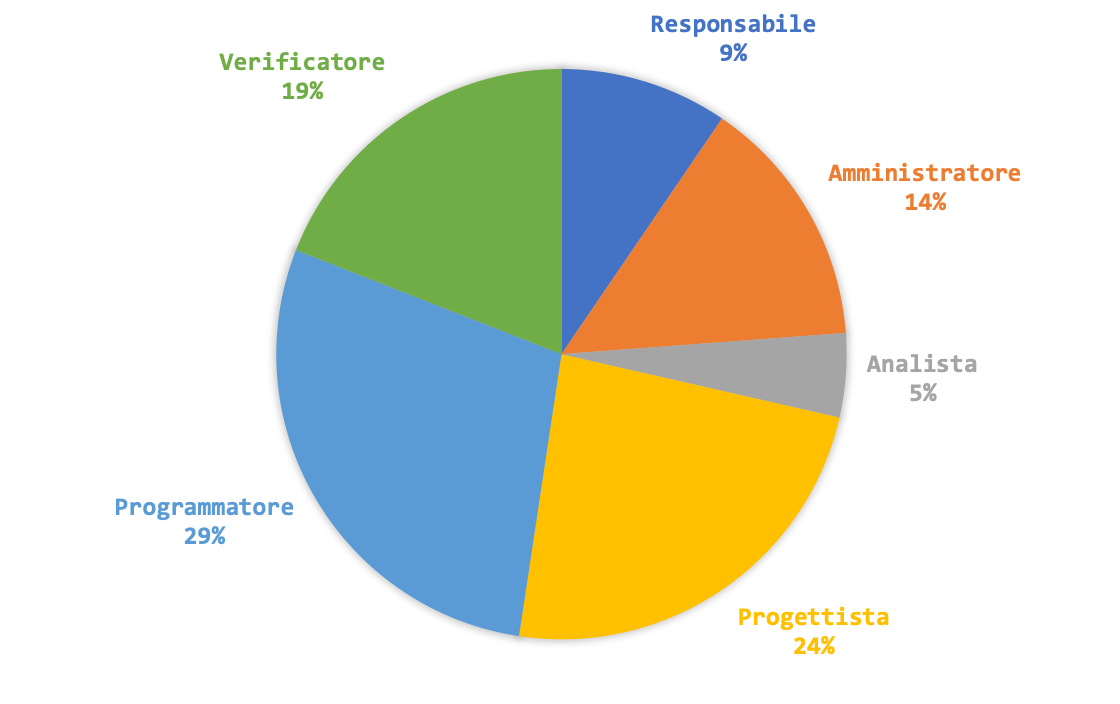
\includegraphics[width=0.8\linewidth]{images/consuntivo/ConsIncr2-2.png}
				\caption{Grafico percentuale ore/ruolo nell'incremento II}
				\label{fig:consuntivo grafico costi ruolo incremento II}
			\end{figure}
			\pagebreak

			\subsubsection*{Conclusioni}
			Durante l'incremento II il gruppo ha lavorato mantenendo il numero di ore che erano state preventivate. È stato necessario però svolgere alcuni cambiamenti nella suddivisione oraria per ruolo, in particolare:
			\begin{itemize}
				\item \textbf{:} 
			\end{itemize}
			Alla luce dei cambiamenti effettuati il risultato è che il gruppo ha ... investendo le stesse ore preventivate.
		

		\subsection{Preventivo a finire}
			A seguito dei cambiamenti riportati .

%%%%%%%%%%%%%%%%%%%%%%%%%%%%%%%%%%%%%%%%%%%%%%%%%%%%%%%%%%%%%%%%%%%%%%%%%%%%%%%%%%%%%%%%%%%%%%%%%%%%%%%%%%%%%%%%%%
		
		\subsection{Incremento III }
		Le ore di lavoro svolte in questo periodo sono volte alla progettazione dell'interfaccia delle \glock{API} ed all'implementazione delle operazioni di lettura dei dati tramite le \glock{API}.
		\subsubsection{Prospetto orario}
			Nella tabella in seguito viene illustrato il cambiamento nel numero d'ore di ogni persona, per ogni ruolo ricoperto:
			
			\rowcolors{2}{lightest-grayest}{white}
			\begin{longtable}{|c|c|c|c|c|c|c|c}
				\hline
				\rowcolor{lighter-grayer}
				\textbf{Nome} & \textbf{Re} & \textbf{Am} & \textbf{An} & \textbf{Pg}  & \textbf{Pr}   & \textbf{Ve} & \textbf{Totale} \\
				\hline
				\endfirsthead
				\hline
				Giuseppe Vito Bitetti & 0 & 0 & 0 & 1 (+1) & 2 (-1) & 3 & 6\\
				\hline
				\hline
				Lorenzo Dei Negri & 0 & 0 & 0 & 3 & 0 & 3 & 6\\
				\hline
				\hline
				Nicolò Frison & 3 & 0 & 0 & 2 & 0 & 1 & 6 \\
				\hline
				\hline
				Fouad Mouad & 0 & 0 & 0 & 3 & 3 & 0 & 6\\
				\hline
				\hline
				Mariano Sciacco & 0 & 3 & 0 & 0 & 3 & 0 & 6 \\
				\hline
				\hline
				Alessandro Tommasin & 0 & 0 & 0 & 2 & 2 & 0 & 6\\
				\hline
				\hline
				Giovanni Vidotto & 0 & 0 & 0 & 3 (+1) & 0 & 3 (-1) & 6 \\
				\hline 
				\textbf{Totale} & 3 &  3 & 0 & 14 (+2) & 10 (-1) & 12 (-1) & 42 \\
				\hline 
				
				\caption{Tabella contenente il prospetto orario preventivato per l'incremento III}
			\end{longtable}
			
			La tabella può essere riassunta nel seguente istogramma:
			
			\begin{figure}[H]
				\centering
				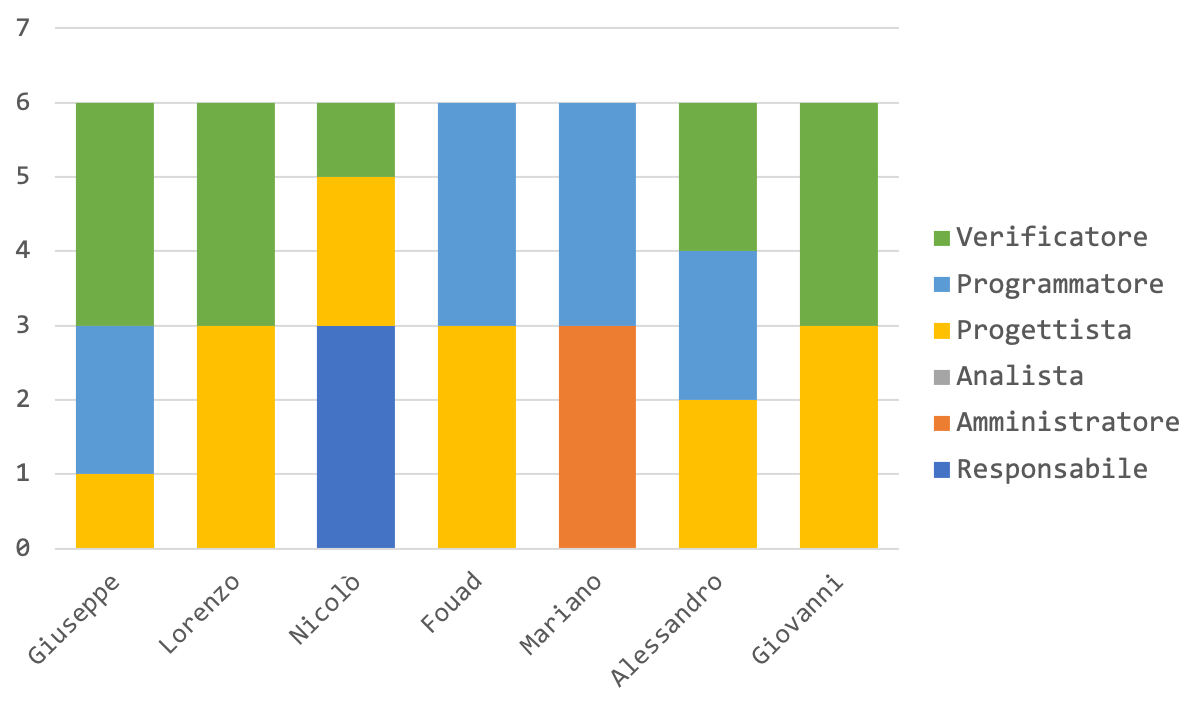
\includegraphics[width=0.8\linewidth]{images/consuntivo/ConsIncr3-1.png}
				\caption{Grafico consuntivo ore/ruolo componenti dell'incremento III}
				\label{fig:consuntivo grafico suddivione ruoli incremento III}
			\end{figure}
			\pagebreak
			
		\subsubsection{Prospetto economico}
			In base al prospetto orario, quello economico sarà il seguente: 
			
			\rowcolors{2}{white}{lightest-grayest}
			\begin{longtable}{|c|c|c|c|c|c|c|c}
				\hline
				\rowcolor{lighter-grayer}
				\textbf{Ruolo} & \textbf{Ore} & \textbf{Costo in €} \\
				\hline
				\endfirsthead
				\hline
			Responsabile 	    & 3 & 90,00 \\
			\hline 
			\hline
			Amministratore	  & 3 & 60,00\\
			\hline
			\hline
			Analista 				& - & -\\
			\hline
			\hline
			Progettista 		  & 14 (+2) & 308,00 (+44,00)\\
			\hline
			\hline
			Programmatore 	 & 10 (-1) & 150,00 (-15,00) \\
			\hline
			\hline
			Verificatore 		  & 12 (-1) & 180,00 (-15,00)\\
			\hline
			\textbf{Totale} 	& 42 & 788,00 (+14,00)\\
			\hline 
				
				\caption{Tabella contenente il prospetto economico in riferimento al prospetto orario}
			\end{longtable}
			
			La tabella può essere riassunta nel seguente areogramma:
			\begin{figure}[H]
				\centering
				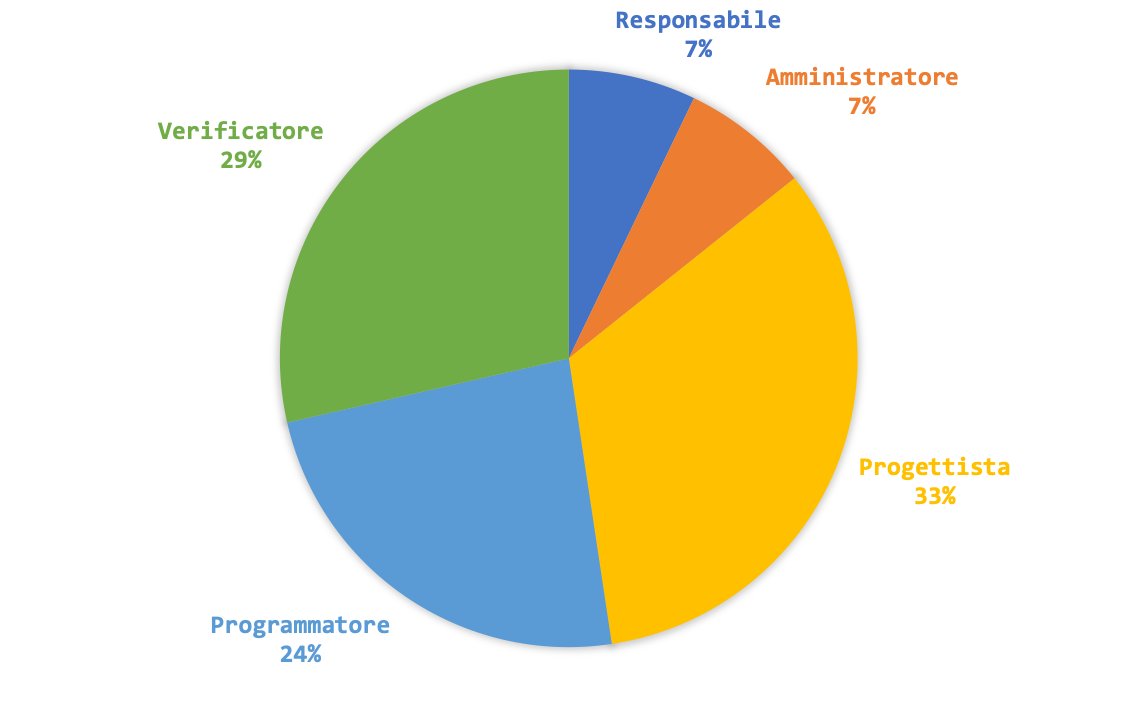
\includegraphics[width=0.8\linewidth]{images/consuntivo/ConsIncr3-2.png}
				\caption{Grafico percentuale ore/ruolo nell'incremento III}
				\label{fig:consuntivo grafico costi ruolo incremento III}
			\end{figure}
			\pagebreak

		\subsubsection*{Conclusioni}
			Durante l'incremento III il gruppo ha lavorato mantenendo il numero di ore che erano state preventivate. È stato necessario però svolgere alcuni cambiamenti nella suddivisione oraria per ruolo, in particolare:
			\begin{itemize}
				\item \textbf{:} 
			\end{itemize}
			Alla luce dei cambiamenti effettuati il risultato è che il gruppo ha ... investendo le stesse ore preventivate.
		

		\subsection{Preventivo a finire}
			A seguito dei cambiamenti riportati .	

		%%%%%%%%%%%%%%%%%%%%%%%%%%%%%%%%%%%%%%%%%%%%%%%%%%%%%%%%%%%%%%%%%%%%%%%%%%%%%%%%%%%%%%%%%%%%%%%%%%%%%%%%%%%%%%%%%%
		
		\subsection{Incremento IV}
		Le ore di lavoro svolte in questo periodo sono volte alla configurazione di base della web app e reperimento dati dalle \glock{API}.
		\subsubsection{Prospetto orario}
			Nella tabella in seguito viene illustrato il cambiamento nel numero d'ore di ogni persona, per ogni ruolo ricoperto:
			
			\rowcolors{2}{lightest-grayest}{white}
			\begin{longtable}{|c|c|c|c|c|c|c|c}
				\hline
				\rowcolor{lighter-grayer}
				\textbf{Nome} & \textbf{Re} & \textbf{Am} & \textbf{An} & \textbf{Pg}  & \textbf{Pr}   & \textbf{Ve} & \textbf{Totale} \\
				\hline
				\endfirsthead
				\hline
				Giuseppe Vito Bitetti & 2 & 0 & 0 & 0 & 4 & 0 & 6\\
				\hline
				\hline
				Lorenzo Dei Negri & 2 & 0 & 0 & 1 (-1) & 0 & 3 (+1) & 6\\
				\hline
				\hline
				Nicolò Frison & 0 & 0 & 0 & 1 (-1) & 4 & 1 (+1) & 6\\
				\hline
				\hline
				Fouad Mouad & 0 & 3 & 0 & 0 & 0 & 3 & 6\\
				\hline
				\hline
				Mariano Sciacco & 3 & 0 & 0 & 0 & 3 & 0 & 6\\
				\hline
				\hline
				Alessandro Tommasin & 0 & 0 & 2 & 0 & 0 & 4 & 6\\
				\hline
				\hline
				Giovanni Vidotto & 0 & 0 & 0 & 5 & 0 & 1 & 6\\
				\hline 
				\textbf{Totale} & 7 &  3 & 4 & 7 (-2) & 11  & 12 (+2) & 42 \\
				\hline 
				
				\caption{Tabella contenente il prospetto orario preventivato per l'incremento IV}
			\end{longtable}
			
			La tabella può essere riassunta nel seguente istogramma:
			
			\begin{figure}[H]
				\centering
				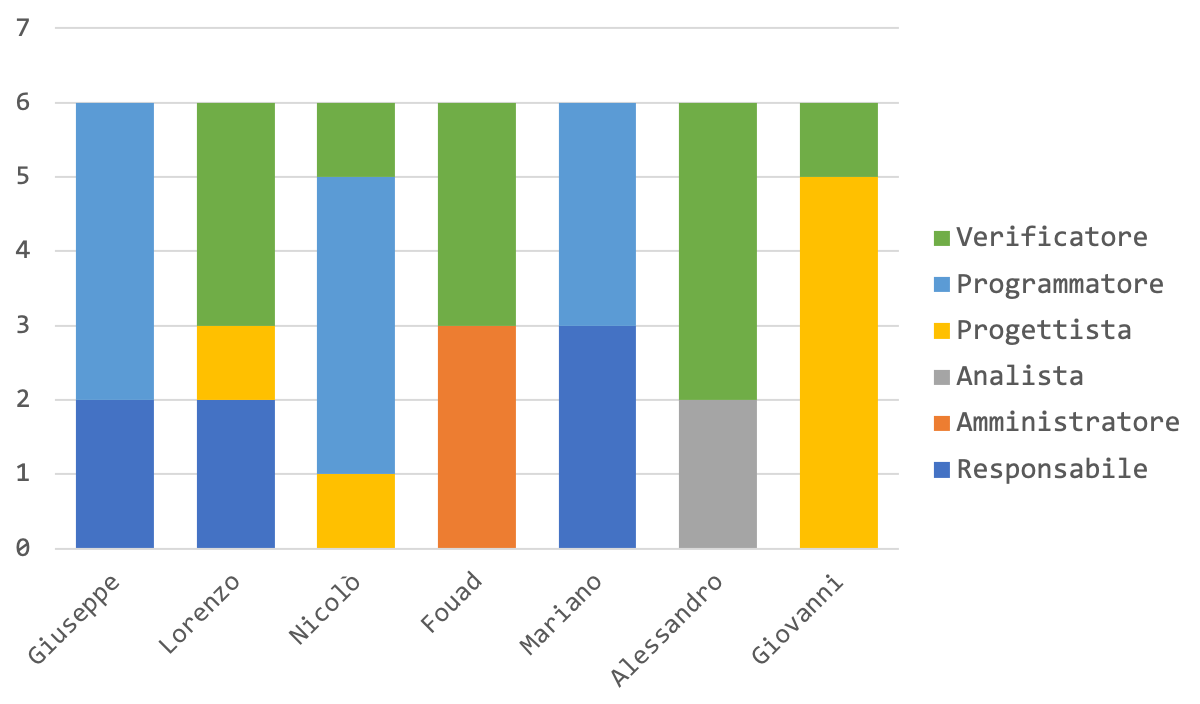
\includegraphics[width=0.8\linewidth]{images/consuntivo/ConsIncr4-1.png}
				\caption{Grafico consuntivo ore/ruolo componenti dell'incremento IV}
				\label{fig:consuntivo grafico suddivisione ruoli incremento IV}
			\end{figure}
			\pagebreak
			
		\subsubsection{Prospetto economico}
			In base al prospetto orario, quello economico sarà il seguente: 
			
			\rowcolors{2}{white}{lightest-grayest}
			\begin{longtable}{|c|c|c|c|c|c|c|c}
				\hline
				\rowcolor{lighter-grayer}
				\textbf{Ruolo} & \textbf{Ore} & \textbf{Costo in €} \\
				\hline
				\endfirsthead
				\hline
			Responsabile 	    & 7 & 210,00\\
			\hline 
			\hline
			Amministratore	  & 3 & 60,00\\
			\hline
			\hline
			Analista 				& 2 & 50,00\\
			\hline
			\hline
			Progettista 		  & 7 (-2) & 154,00 (-44,00)\\
			\hline
			\hline
			Programmatore 	 & 11 & 165,00\\
			\hline
			\hline
			Verificatore 		  & 10 (+2) & 180,00 (+30,00) \\
			\hline
			\textbf{Totale} 	& 42 & 819,00 (-14,00)\\
			\hline
				
				\caption{Tabella contenente il prospetto economico in riferimento al prospetto orario}
			\end{longtable}
			
			La tabella può essere riassunta nel seguente areogramma:
			\begin{figure}[H]
				\centering
				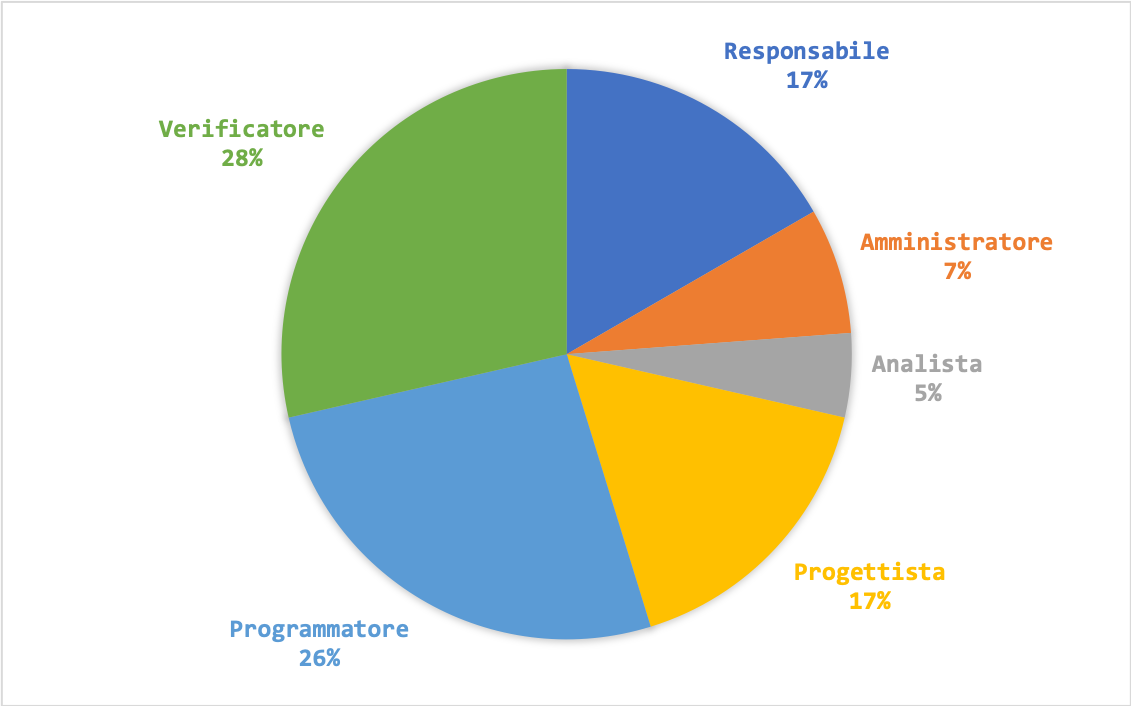
\includegraphics[width=0.8\linewidth]{images/consuntivo/ConsIncr4-2.png}
				\caption{Grafico percentuale ore/ruolo nell'incremento IV}
				\label{fig:consuntivo grafico costi ruolo incremento IV}
			\end{figure}
			\pagebreak	
		\subsubsection*{Conclusioni}
			Durante l'incremento IV il gruppo ha lavorato mantenendo il numero di ore che erano state preventivate. È stato necessario però svolgere alcuni cambiamenti nella suddivisione oraria per ruolo, in particolare:
			\begin{itemize}
				\item \textbf{:} 
			\end{itemize}
			Alla luce dei cambiamenti effettuati il risultato è che il gruppo ha ... investendo le stesse ore preventivate.
		

		\subsection{Preventivo a finire}
			A seguito dei cambiamenti riportati .


		%%%%%%%%%%%%%%%%%%%%%%%%%%%%%%%%%%%%%%%%%%%%%%%%%%%%%%%%%%%%%%%%%%%%%%%%%%%%%%%%%%%%%%%%%%%%%%%%%%%%%%%%%%%%%%%%%%
		
		\subsection{Incremento V }
		Le ore di lavoro svolte in questo periodo sono volte all'implementazione della configurazione dinamica di un \glock{gateway}.
		\subsubsection{Prospetto orario}
			Nella tabella in seguito viene illustrato il cambiamento nel numero d'ore di ogni persona, per ogni ruolo ricoperto:
			
			\rowcolors{2}{lightest-grayest}{white}
			\begin{longtable}{|c|c|c|c|c|c|c|c}
				\hline
				\rowcolor{lighter-grayer}
				\textbf{Nome} & \textbf{Re} & \textbf{Am} & \textbf{An} & \textbf{Pg}  & \textbf{Pr}   & \textbf{Ve} & \textbf{Totale} \\
				\hline
				\endfirsthead
				\hline
				Giuseppe Vito Bitetti & 0 & 2 & 2 & 0 & 0 & 2 & 6\\
				\hline
				\hline
				Lorenzo Dei Negri & 0 & 0 & 0 & 2 & 4 & 0 & 6\\
				\hline
				\hline
				Nicolò Frison & 2 & 0 & 0 & 0 & 0 & 4 & 6\\
				\hline
				\hline
				Fouad Mouad & 3 (+1) & 0 & 0 & 0 & 3 (-1) & 0 & 6 \\
				\hline
				\hline
				Mariano Sciacco & 0 & 0 & 0 & 3(+2) & 3 & 0(-2) & 6\\
				\hline
				\hline
				Alessandro Tommasin & 0 & 0 & 0 & 3 & 3 & 0 & 6\\
				\hline
				\hline
				Giovanni Vidotto & 0 & 2 & 0 & 0 & 4 & 0 & 6\\
				\hline 
				\textbf{Totale} & 5 (+1) & 4 & 2 & 8 (+2) & 17 (-1) & 6(-2) & 42 \\
				\hline 
				
				\caption{Tabella contenente il prospetto orario preventivato per l'incremento V}
			\end{longtable}	
			
			La tabella può essere riassunta nel seguente istogramma:
			
			\begin{figure}[H]
				\centering
				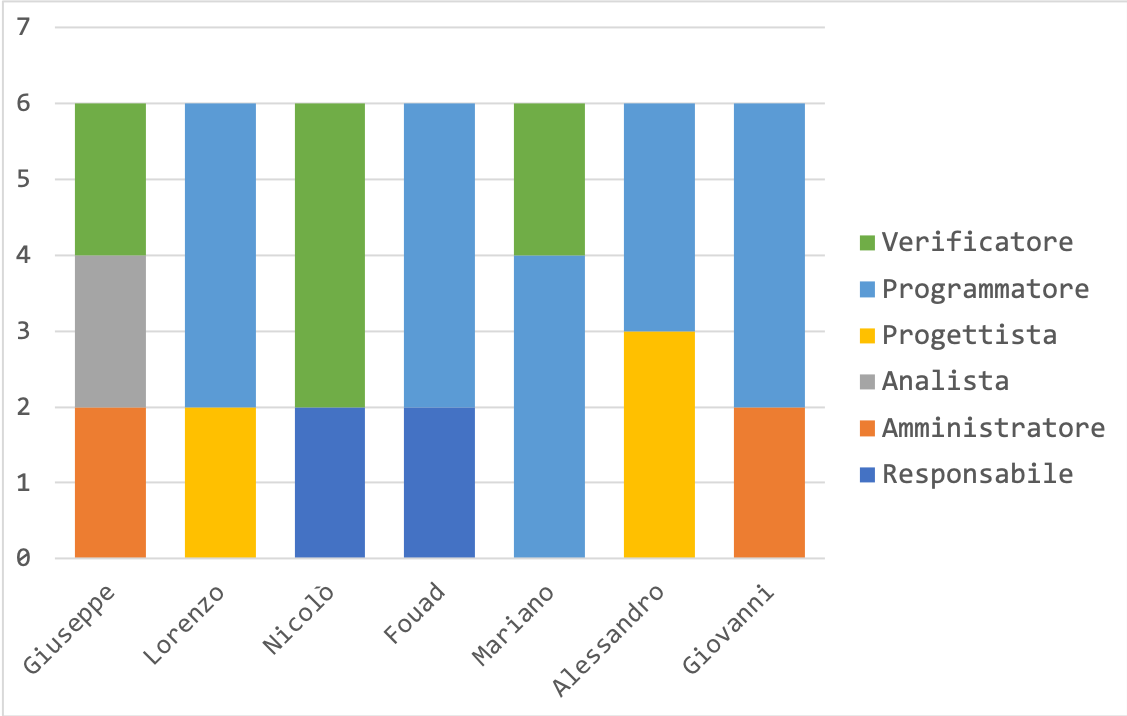
\includegraphics[width=0.8\linewidth]{images/consuntivo/ConsIncr5-1.png}
				\caption{Grafico consuntivo ore/ruolo componenti dell'incremento V}
				\label{fig:consuntivo grafico suddivisione ruoli incremento V}
			\end{figure}
			\pagebreak
			
		\subsubsection{Prospetto economico}
			In base al prospetto orario, quello economico sarà il seguente: 
			
			\rowcolors{2}{white}{lightest-grayest}
			\begin{longtable}{|c|c|c|c|c|c|c|c}
				\hline
				\rowcolor{lighter-grayer}
				\textbf{Ruolo} & \textbf{Ore} & \textbf{Costo in €} \\
				\hline
				\endfirsthead
				\hline
			Responsabile 	    & 5 (+1) & 150,00 (+30,00)\\
			\hline 
			\hline
			Amministratore	  & 4 & 80,00\\
			\hline
			\hline
			Analista 				& 2 & 50,00\\
			\hline
			\hline
			Progettista 		  & 8 (+2) & 176,00 (+44,00)\\
			\hline
			\hline
			Programmatore 	 & 17 (-1)  & 255 (-15),00 \\
			\hline
			\hline
			Verificatore 		  & 6 (-2) & 90,00 (-30)\\
			\hline
			\textbf{Totale} 	&  42 & 801,00 (+29,00)\\
			\hline
				
				\caption{Tabella contenente il prospetto economico in riferimento al prospetto orario}
			\end{longtable}
			
			La tabella può essere riassunta nel seguente areogramma:
			\begin{figure}[H]
				\centering
				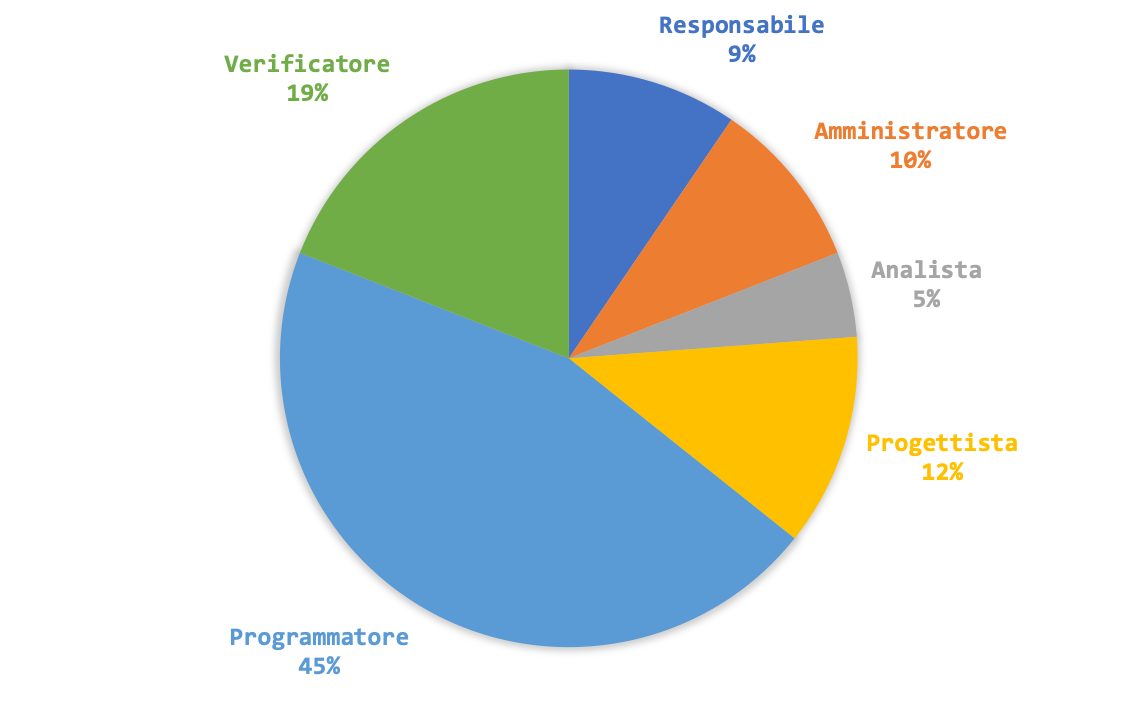
\includegraphics[width=0.8\linewidth]{images/consuntivo/ConsIncr5-2.png}
				\caption{Grafico percentuale ore/ruolo nell'incremento V}
				\label{fig:consuntivo grafico costi ruolo incremento V}
			\end{figure}

		%Conclusioni per la revisione di progettazione
		\subsubsection*{Conclusioni}
			Durante il periodo che va dall'inizio della fase di progettazione della technology baseline all'ultimo incremento prima della revisione di progettazione il gruppo ha lavorato mantenendo il numero di ore che erano state preventivate. È stato necessario però svolgere alcuni cambiamenti nella suddivisione oraria per ruolo, in particolare:
			\begin{itemize}
				\item \textbf{responsabile:} sono state impiegate meno ore rispetto a quelle preventivate, in quanto nel piano di progetto e nell'approvazione dei documenti sono stati riscontrate meno difficoltà del previsto;
				\item \textbf{progettista:} sono state richieste più ore di quelle preventivate poiché il gruppo ha riscontrato alcune difficoltà nello svolgimento di questo ruolo;
				\item \textbf{verificatore:} è stato richiesto un quantitativo maggiore di ore rispetto a ciò che era stato preventivato per assicurare la correttezza e la qualità del lavoro svolto.
			\end{itemize}
			Alla luce dei cambiamenti effettuati il risultato è che il gruppo ha risparmiato 1,00 € investendo le stesse ore preventivate.
		

		\subsection{Preventivo a finire}
			A seguito dei cambiamenti riportati, non sono stati ritenuti necessari dei provvedimenti per quanto riguarda il piano economico, in quanto non è stato sforato il budget preventivato, nonostante i cambiamenti orari che si sono verificati.
			
			% Di seguito il preventivo a finire:
			% \rowcolors{2}{white}{lightest-grayest}
			% \begin{longtable}{|c|c|c|c|c|c|c|c}
			% 	\hline
			% 	\rowcolor{lighter-grayer}
			% 	\textbf{Fase} & \textbf{Preventivo in €} & \textbf{consuntivo in €} \\
			% 	\hline
			%	\endfirsthead
			% 	
			% 	\hline
			% 	Analisi & 4.410,00 & 4.390,00\\
			% 	\hline
			% 	\hline
			% 	\textbf{Totale rendicontato} & 13.806,00 & 13.806,00\\
			% 	\hline
			% 	\hline
			% 	\textbf{Totale} & 18.966,00 & 18.966,00\\
			% 	\hline
			% 	\caption{Tabella contenente il preventivo a finire}
			% \end{longtable}
			
			
			